\documentclass[
border=10pt,
varwidth=24cm
]{standalone}

\usepackage[T1]{fontenc}
\usepackage[utf8]{inputenc}
\usepackage{lmodern}
\usepackage{array}
\usepackage{amsmath}
\usepackage{amssymb}
\usepackage{tikz}

\usetikzlibrary{calc}
\usetikzlibrary{shapes.geometric}

\setlength{\parindent}{0pt}
\setlength{\tabcolsep}{4pt}
\renewcommand{\arraystretch}{1.25}
\setlength{\extrarowheight}{4pt}

% Paragraph columns: top-aligned text, no paragraph indentation.
\newcolumntype{L}[1]{>{\raggedright\arraybackslash\setlength{\parindent}{0pt}\setlength{\parskip}{0pt}}p{#1}}

% Centered paragraph columns.
\newcolumntype{C}[1]{>{\centering\arraybackslash\setlength{\parindent}{0pt}\setlength{\parskip}{0pt}}p{#1}}

% Vertically and horizontally centered columns.
% Used for the # and Marks columns.
\newcolumntype{M}[1]{>{\centering\arraybackslash\setlength{\parindent}{0pt}\setlength{\parskip}{0pt}}m{#1}}

% Center content inside an answer column without display-math vertical spacing.
\newcommand{\AnswerCenter}[1]{%
	\makebox[\linewidth][c]{#1}%
}

% Default helper height used explicitly in selected rows.
\newcommand{\QFourHeight}{4.25cm}

\newcommand{\CellCenter}[2]{%
	\begin{minipage}[t][#1][c]{\linewidth}
		\centering
		#2
	\end{minipage}%
}

\newcommand{\CellTop}[2]{%
	\begin{minipage}[t][#1][t]{\linewidth}
		\raggedright
		#2
	\end{minipage}%
}

\newcommand{\tallyfive}{%
	\ensuremath{%
		\vcenter{\hbox{%
				\tikz[x=0.68ex, y=0.52ex]{
					% Balanced invisible box for centering
					\useasboundingbox (-0.5,-0.2) rectangle (3.5,4.2);
					
					% Four vertical tally marks
					\draw[line width=0.45pt, line cap=round] (0,0) -- (0,4);
					\draw[line width=0.45pt, line cap=round] (1,0) -- (1,4);
					\draw[line width=0.45pt, line cap=round] (2,0) -- (2,4);
					\draw[line width=0.45pt, line cap=round] (3,0) -- (3,4);
					
					% Diagonal crossing stroke
					\draw[line width=0.45pt, line cap=round] (-0.35,0.75) -- (3.35,3.25);
				}%
		}}%
	}%
}

\begin{document}
	
	\begin{center}
		{\Large\bfseries Cambridge -- Mathematics -- Stage 4 -- Paper 2}
	\end{center}
	
	\vspace{0.4cm}
	
	\begin{tabular}{|M{0.95cm}|L{7.4cm}|M{1.05cm}|L{3.6cm}|L{5.2cm}|}
		\hline
		\textbf{\#}
		& \multicolumn{1}{c|}{\textbf{Answer}}
		& \textbf{Marks}
		& \multicolumn{1}{c|}{\textbf{Part Marks}}
		& \multicolumn{1}{c|}{\textbf{Guidance}} \\
		\hline
		
		1 & Three thousand & 1 & &
		Accept 3 thousands.
		
		Do not accept 3 000.
		
		Do not accept `thousand' without the 3. \\
		\hline
		\CellCenter{1.5cm}{2} &
		\CellCenter{1.5cm}{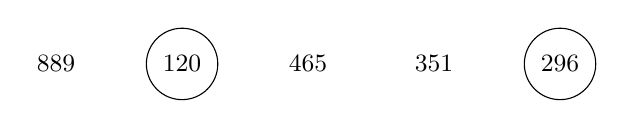
\begin{tikzpicture}[scale=1, every node/.style={font=\small, transform shape}]
			\node at (0,0) {889};
			\node[draw, circle, inner sep=4pt] at (1.6,0) {120};
			\node at (3.2,0) {465};
			\node at (4.8,0) {351};
			\node[draw, circle, inner sep=4pt] at (6.4,0) {296};
		\end{tikzpicture}}
		& \CellCenter{1.5cm}{1} &
		&
		Both answers correct for the mark.
		Accept any clear indication. \\
		\hline
		
		3 &
		\AnswerCenter{%
			\(\displaystyle
			\frac{6}{5}
			\qquad
			\frac{5}{10}
			\)
		}
		& 2 &
		Award 1 mark for each correct answer.
		&
		Accept equivalent answers. \\
		\hline
		
		\CellCenter{\QFourHeight}{4}
		&
		\CellCenter{\QFourHeight}{%
			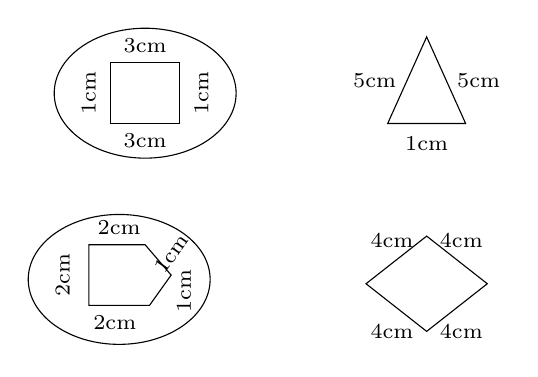
\begin{tikzpicture}[scale=1.1, every node/.style={font=\scriptsize, transform shape}]
				% Top-left circled rectangle
				\draw (1.4,2.9) ellipse (1.05 and 0.75);
				\draw (1.0,2.55) rectangle (1.8,3.25);
				\node at (1.4,3.45) {\(3\mathrm{cm}\)};
				\node at (1.4,2.35) {\(3\mathrm{cm}\)};
				\node[rotate=90] at (0.75,2.9) {\(1\mathrm{cm}\)};
				\node[rotate=90] at (2.05,2.9) {\(1\mathrm{cm}\)};
				
				% Top-right triangle
				\draw (4.2,2.55) -- (5.1,2.55) -- (4.65,3.55) -- cycle;
				\node at (4.05,3.05) {\(5\mathrm{cm}\)};
				\node at (5.25,3.05) {\(5\mathrm{cm}\)};
				\node at (4.65,2.32) {\(1\mathrm{cm}\)};
				
				% Bottom-left circled irregular polygon
				\draw (1.1,0.75) ellipse (1.05 and 0.75);
				\draw (0.75,0.45) -- (1.45,0.45) -- (1.70,0.80) -- (1.40,1.15) -- (0.75,1.15) -- cycle;
				\node at (1.10,1.35) {\(2\mathrm{cm}\)};
				\node[rotate=90] at (0.45,0.80) {\(2\mathrm{cm}\)};
				\node at (1.05,0.25) {\(2\mathrm{cm}\)};
				\node[rotate=55] at (1.70,1.05) {\(1\mathrm{cm}\)};
				\node[rotate=90] at (1.85,0.62) {\(1\mathrm{cm}\)};
				
				% Bottom-right rhombus
				\draw (4.65,1.25) -- (5.35,0.70) -- (4.65,0.15) -- (3.95,0.70) -- cycle;
				\node at (4.25,1.20) {\(4\mathrm{cm}\)};
				\node at (5.05,1.20) {\(4\mathrm{cm}\)};
				\node at (4.25,0.15) {\(4\mathrm{cm}\)};
				\node at (5.05,0.15) {\(4\mathrm{cm}\)};
			\end{tikzpicture}%
		}
		&
		\CellCenter{\QFourHeight}{1}
		&
		&
		\CellTop{\QFourHeight}{%
			Both answers correct for the mark.
			
			Accept any clear indication.
		} \\
		\hline
		
		\CellCenter{\QFourHeight}{5}
		&
		\CellCenter{\QFourHeight}{%
			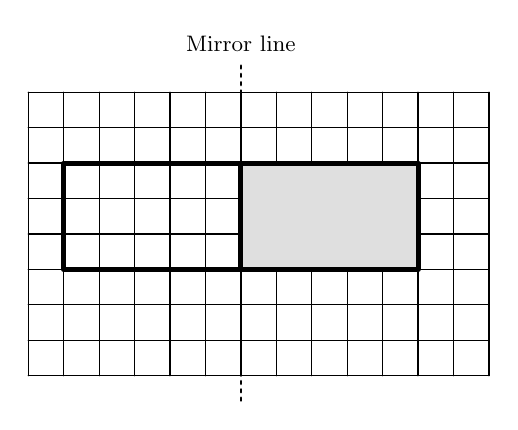
\begin{tikzpicture}[
				scale=0.45,
				line cap=round,
				line join=round,
				every node/.style={font=\small, transform shape}
				]
				% Grid
				\draw[step=1, line width=0.45pt] (0,0) grid (13,8);
				
				% Mirror-image rectangle on the left
				\draw[line width=1.8pt] (1,3) rectangle (6,6);
				
				% Shaded rectangle on the right
				\fill[gray!25] (6,3) rectangle (11,6);
				\draw[line width=1.8pt] (6,3) rectangle (11,6);
				
				% Mirror line
				\draw[dotted, line width=1pt] (6,-0.7) -- (6,8.9);
				
				% Mirror line label
				\node[above, scale=2, transform shape] at (6,8.9) {Mirror line};
			\end{tikzpicture}%
		}
		&
		\CellCenter{\QFourHeight}{1}
		&
		&
		\CellTop{\QFourHeight}{Accept slight inaccuracies provided the intention is clear.} \\
		\hline
		
		6 & 92 546 & 1 & & Accept any clear indication. \\
		\hline
		
		\CellCenter{\QFourHeight}{7}
		&
		\CellCenter{\QFourHeight}{%
			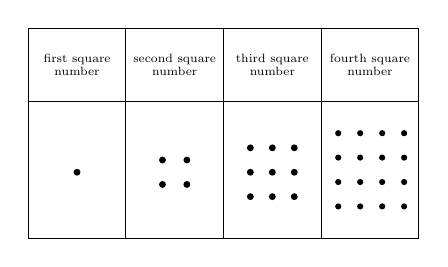
\begin{tikzpicture}[scale=0.62, every node/.style={font=\scriptsize, transform shape}]
				% Table border and grid
				\draw (0,0) rectangle (8,4.3);
				\draw (2,0) -- (2,4.3);
				\draw (4,0) -- (4,4.3);
				\draw (6,0) -- (6,4.3);
				\draw (0,2.8) -- (8,2.8);
				
				% Headings
				\node[align=center] at (1,3.55) {first square\\number};
				\node[align=center] at (3,3.55) {second square\\number};
				\node[align=center] at (5,3.55) {third square\\number};
				\node[align=center] at (7,3.55) {fourth square\\number};
				
				% First square number: 1
				\fill (1,1.35) circle (2pt);
				
				% Second square number: 4
				\foreach \x in {2.75,3.25}
				\foreach \y in {1.10,1.60}
				\fill (\x,\y) circle (2pt);
				
				% Third square number: 9
				\foreach \x in {4.55,5.00,5.45}
				\foreach \y in {0.85,1.35,1.85}
				\fill (\x,\y) circle (2pt);
				
				% Fourth square number: 16
				\foreach \x in {6.35,6.80,7.25,7.70}
				\foreach \y in {0.65,1.15,1.65,2.15}
				\fill (\x,\y) circle (1.8pt);
			\end{tikzpicture}%
		}
		&
		\CellCenter{\QFourHeight}{1}
		&
		&
		Accept slight inaccuracies provided the intention is clear. \\
		\hline
		
		8 &
		\begin{tabular}[t]{@{}l@{}}
			8300 \\
			523
		\end{tabular}
		& 1 &
		&
		Both answers correct for the mark. \\
		\hline
		
		\CellCenter{6.5cm}{9}
		&
		\CellCenter{6.5cm}{%
			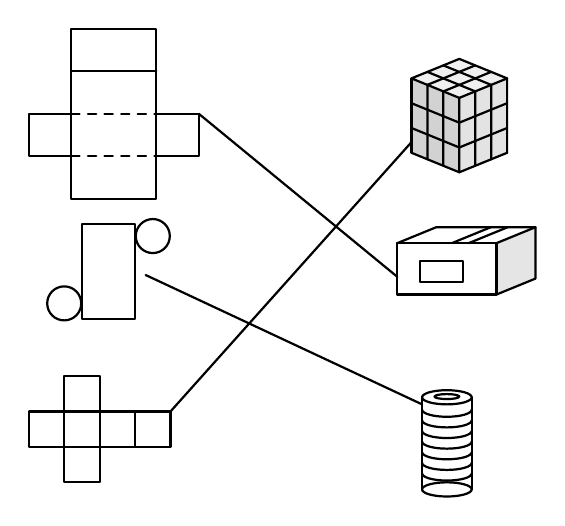
\begin{tikzpicture}[
				line cap=round,
				line join=round,
				draw=black,
				thick,
				fold/.style={dashed, thick},
				match/.style={thick},
				scale=0.45
				]
				% Rectangular prism net
				\begin{scope}[shift={(0,7.2)}]
					\draw (1.2,-1.2) rectangle (3.6,2.4);
					\draw (0,0) rectangle (1.2,1.2);
					\draw (3.6,0) rectangle (4.8,1.2);
					\draw (1.2,2.4) rectangle (3.6,3.6);
					
					\draw[fold] (1.2,0) -- (3.6,0);
					\draw[fold] (1.2,1.2) -- (3.6,1.2);
					\draw[fold] (1.2,2.4) -- (3.6,2.4);
					\draw[fold] (1.2,0) -- (1.2,1.2);
					\draw[fold] (3.6,0) -- (3.6,1.2);
				\end{scope}
				
				% Cylinder net
				\begin{scope}[shift={(0.5,2.6)}]
					\draw (1,0) rectangle (2.5,2.7);
					\draw (0.5,0.45) circle (0.48);
					\draw (3.0,2.35) circle (0.48);
				\end{scope}
				
				% Cube net
				\begin{scope}[shift={(0,-1)}]
					\foreach \x in {0,1,2,3}
					\draw (\x,0) rectangle ++(1,1);
					
					\draw (1,1) rectangle ++(1,1);
					\draw (1,-1) rectangle ++(1,1);
					
					\draw[fold] (1,0) -- (1,1);
					\draw[fold] (2,0) -- (2,1);
					\draw[fold] (3,0) -- (3,1);
					\draw[fold] (1,1) -- (2,1);
					\draw[fold] (1,0) -- (2,0);
				\end{scope}
				
				% Cube
				\begin{scope}[shift={(10.8,9.4)}]
					\coordinate (A) at (0,0);
					\coordinate (B) at (1.35,0.55);
					\coordinate (C) at (2.70,0);
					\coordinate (D) at (1.35,-0.55);
					
					\coordinate (Av) at ($(A)+(0,-2.1)$);
					\coordinate (Cv) at ($(C)+(0,-2.1)$);
					\coordinate (Dv) at ($(D)+(0,-2.1)$);
					
					\fill[gray!12] (A) -- (B) -- (C) -- (D) -- cycle;
					\fill[gray!35] (A) -- (D) -- (Dv) -- (Av) -- cycle;
					\fill[gray!22] (D) -- (C) -- (Cv) -- (Dv) -- cycle;
					
					\draw (A) -- (B) -- (C) -- (D) -- cycle;
					\draw (A) -- (Av);
					\draw (D) -- (Dv);
					\draw (C) -- (Cv);
					\draw (Av) -- (Dv) -- (Cv);
					
					\foreach \t in {1/3,2/3}{
						\draw ($(A)!\t!(B)$) -- ($(D)!\t!(C)$);
						\draw ($(A)!\t!(D)$) -- ($(B)!\t!(C)$);
						
						\draw ($(A)!\t!(D)$) -- ($(Av)!\t!(Dv)$);
						\draw ($(A)!\t!(Av)$) -- ($(D)!\t!(Dv)$);
						
						\draw ($(D)!\t!(C)$) -- ($(Dv)!\t!(Cv)$);
						\draw ($(D)!\t!(Dv)$) -- ($(C)!\t!(Cv)$);
					}
				\end{scope}
				
				% Rectangular prism
				\begin{scope}[shift={(10.4,3.3)}]
					\coordinate (A) at (0,0);
					\coordinate (B) at (2.8,0);
					\coordinate (C) at (2.8,1.45);
					\coordinate (D) at (0,1.45);
					\coordinate (v) at (1.1,0.45);
					
					\coordinate (E) at ($(B)+(v)$);
					\coordinate (F) at ($(C)+(v)$);
					\coordinate (G) at ($(D)+(v)$);
					
					\fill[gray!20] (B)--(E)--(F)--(C)--cycle;
					\draw (A)--(B)--(C)--(D)--cycle;
					\draw (B)--(E)--(F)--(C);
					\draw (D)--(G)--(F);
					
					\draw ($(D)!0.55!(C)$)--($(G)!0.55!(F)$);
					\draw ($(D)!0.72!(C)$)--($(G)!0.72!(F)$);
					\draw (0.65,0.35) rectangle (1.85,0.95);
				\end{scope}
				
				% Cylinder
				\begin{scope}[shift={(11.8,0.4)}]
					\def\rx{0.7}
					\def\ry{0.2}
					\def\h{2.6}
					
					\draw (0,0) ellipse[x radius=\rx,y radius=\ry];
					\draw (-\rx,0) -- (-\rx,-\h);
					\draw (\rx,0) -- (\rx,-\h);
					\draw (0,-\h) ellipse[x radius=\rx,y radius=\ry];
					
					\foreach \y in {-0.35,-0.65,-0.95,-1.25,-1.55,-1.85,-2.15}
					\draw (-\rx,\y) arc[start angle=180,end angle=360,x radius=\rx,y radius=\ry];
					
					\draw (0,0.02) ellipse[x radius=0.35,y radius=0.07];
				\end{scope}
				
				% Matching lines
				\draw[match] (4.8,8.4) -- (10.4,3.8);
				\draw[match] (3.3,3.85) -- (11.1,0.2);
				\draw[match] (4,0) -- (10.8,7.6);
			\end{tikzpicture}%
		}
		&
		\CellCenter{6.5cm}{1}
		&
		&
		\CellTop{6.5cm}{%
			All three lines correct for the mark.
			
			\vspace{0.2cm}
			Accept any clear indication.
		} \\
		\hline
		
		10(a) & 319 & 1 & & \\
		\hline
		
		10(b) & 376 (passengers) & 1 & & \\
		\hline
		
		11 &
		Ages of children in her school
		
		Heights of children in her school
		& 1 &
		&
		Both answers correct in either order for the mark. \\
		\hline
		
		\CellCenter{5cm}{12}
		&
		\CellCenter{5cm}{%
			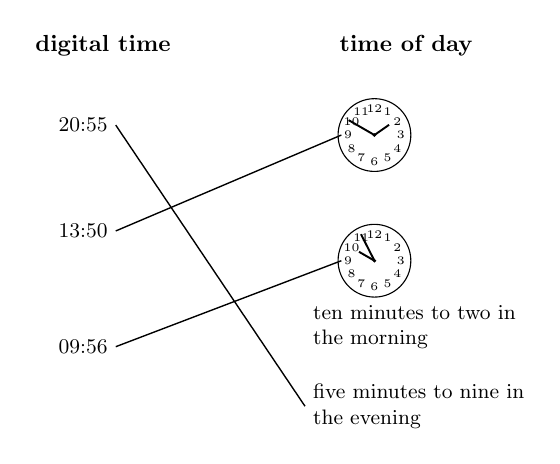
\begin{tikzpicture}[scale=0.84, every node/.style={font=\small, transform shape}]
				\node[font=\bfseries, anchor=west] at (0,5.8) {digital time};
				\node[font=\bfseries, anchor=west] at (4.6,5.8) {time of day};
				
				\node[anchor=west] (t1) at (0.35,4.6) {20:55};
				\node[anchor=west] (t2) at (0.35,3.0) {13:50};
				\node[anchor=west] (t3) at (0.35,1.25) {09:56};
				
				\begin{scope}[shift={(5.25,4.45)}]
					\draw (0,0) circle (0.55);
					\foreach \a/\n in {
						90/12,60/1,30/2,0/3,-30/4,-60/5,-90/6,
						-120/7,-150/8,180/9,150/10,120/11
					}
					\node[font=\tiny] at (\a:0.40) {\n};
					\draw[line width=0.7pt] (0,0) -- (150:0.45);
					\draw[line width=0.7pt] (0,0) -- (35:0.27);
					\fill (0,0) circle (0.03);
				\end{scope}
				
				\begin{scope}[shift={(5.25,2.55)}]
					\draw (0,0) circle (0.55);
					\foreach \a/\n in {
						90/12,60/1,30/2,0/3,-30/4,-60/5,-90/6,
						-120/7,-150/8,180/9,150/10,120/11
					}
					\node[font=\tiny] at (\a:0.40) {\n};
					\draw[line width=0.7pt] (0,0) -- (150:0.27);
					\draw[line width=0.7pt] (0,0) -- (117:0.45);
					\fill (0,0) circle (0.03);
				\end{scope}
				
				\node[align=left, anchor=west] (w1) at (4.2,1.55)
				{ten minutes to two in\\the morning};
				
				\node[align=left, anchor=west] (w2) at (4.2,0.35)
				{five minutes to nine in\\the evening};
				
				\draw[line width=0.5pt] (t2.east) -- (4.75,4.45);
				\draw[line width=0.5pt] (t3.east) -- (4.75,2.55);
				\draw[line width=0.5pt] (t1.east) -- (w2.west);
			\end{tikzpicture}%
		}
		&
		\CellCenter{5cm}{1}
		&
		&
		\CellTop{\QFourHeight}{Award 1 mark for three correct lines drawn.} \\
		\hline
		
		13 &
		\vspace{-10mm}
		\CellCenter{\QFourHeight}{\begin{tabular}[t]{@{}l@{}}
			Line drawn at 750 ml \\[0.15cm]
			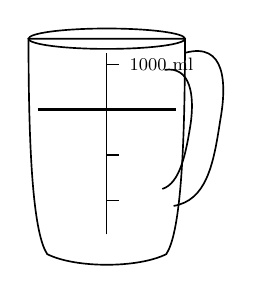
\begin{tikzpicture}[scale=0.72, every node/.style={font=\small, transform shape}]
				% Jar body
				\draw[line width=0.6pt]
				(0.95,0.20)
				.. controls (0.72,0.55) and (0.62,1.80) .. (0.62,4.00)
				-- (3.38,4.00)
				.. controls (3.38,1.80) and (3.28,0.55) .. (3.05,0.20)
				.. controls (2.55,-0.05) and (1.45,-0.05) .. (0.95,0.20)
				-- cycle;
				
				% Jar opening
				\draw[line width=0.6pt] (2.00,4.00) ellipse (1.38 and 0.18);
				
				% Handle
				\draw[line width=0.6pt]
				(3.38,3.75)
				.. controls (4.10,3.95) and (4.12,3.20) .. (4.00,2.55)
				.. controls (3.88,1.75) and (3.75,1.15) .. (3.18,1.05);
				\draw[line width=0.6pt]
				(3.02,3.45)
				.. controls (3.48,3.52) and (3.55,3.00) .. (3.48,2.50)
				.. controls (3.40,2.00) and (3.30,1.45) .. (2.98,1.35);
				
				% Central guide and 4 evenly spaced ticks
				\draw[line width=0.5pt] (2.00,0.55) -- (2.00,3.75);
				\foreach \y in {1.15,1.95,2.75,3.55}
				\draw[line width=0.45pt] (2.00,\y) -- (2.22,\y);
				
				% Top label
				\node[anchor=west] at (2.28,3.55) {1000 ml};
				
				% Liquid level / line drawn at 750 ml (3rd tick)
				\draw[line width=0.8pt] (0.78,2.75) -- (3.22,2.75);
			\end{tikzpicture}
		\end{tabular}}
		& \CellCenter{\QFourHeight}{1} &
		&
		\CellTop{\QFourHeight}{Accept slight inaccuracies provided the intention is clear.} \\
		\hline
		
		\CellCenter{1cm}{14} &
		\CellCenter{1cm}{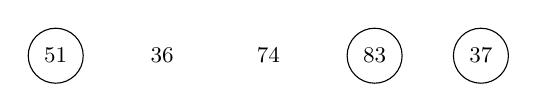
\begin{tikzpicture}[scale=0.9, every node/.style={font=\small, transform shape}]
			\node[draw, circle, inner sep=4pt] at (0,0) {51};
			\node at (1.5,0) {36};
			\node at (3.0,0) {74};
			\node[draw, circle, inner sep=4pt] at (4.5,0) {83};
			\node[draw, circle, inner sep=4pt] at (6.0,0) {37};
		\end{tikzpicture}}
		& \CellCenter{1cm}{1} &
		&
		\CellTop{1cm}{Award 1 mark for all three correct answers.
	
		Accept any clear indication.} \\
		\hline
		
		\CellCenter{\QFourHeight}{15} &
		\CellCenter{\QFourHeight}{\begin{tabular}{|c|c|c|}
			\cline{2-3}
			\multicolumn{1}{c|}{} &
			\begin{tabular}{c}
				equivalent to \(\dfrac{1}{5}\)
			\end{tabular}
			&
			\begin{tabular}{c}
				not equivalent to \(\dfrac{1}{5}\)
			\end{tabular}
			\\
			\hline
			\(\dfrac{2}{10}\) & \(\checkmark\) & \\
			\hline
			\(\dfrac{3}{12}\) & & \(\checkmark\) \\
			\hline
			\(\dfrac{4}{15}\) & & \(\checkmark\) \\
			\hline
			\(\dfrac{5}{25}\) & \(\checkmark\) & \\
			\hline
		\end{tabular}}
		& \CellCenter{\QFourHeight}{1} &
		&
		\CellTop{\QFourHeight}{All four ticks correct for the mark.
		
		\vspace{0.2cm}
		Accept any clear indication.} \\
		\hline
		
		16 & Any number from 45 000 to 54 999 inclusive. & 1 & & \\
		\hline
		
		17(a) & 32 (minutes) & 1 & & \\
		\hline
		
		17(b) & 15:45 & 1 & &
		Accept equivalent correctly converted times, e.g. 3.45 pm \\
		\hline
		
		18(a) & 14 & 1 & & \\
		\hline
		
		18(b) & 18 & 1 & & \\
		\hline
		
		19 & 21 (sweets) & 1 & & \\
		\hline
		
		\CellCenter{\QFourHeight}{20} &
		\CellCenter{\QFourHeight}{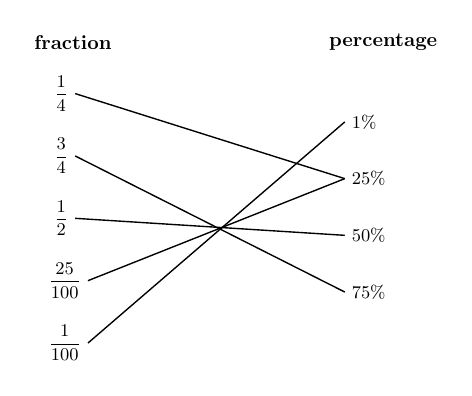
\begin{tikzpicture}[scale=0.72, every node/.style={font=\small, transform shape}]
			\node[font=\bfseries, anchor=west] at (0,5.2) {fraction};
			\node[font=\bfseries, anchor=west] at (5.2,5.2) {percentage};
			
			\node[anchor=west] (f1) at (0.35,4.3) {\(\dfrac{1}{4}\)};
			\node[anchor=west] (f2) at (0.35,3.2) {\(\dfrac{3}{4}\)};
			\node[anchor=west] (f3) at (0.35,2.1) {\(\dfrac{1}{2}\)};
			\node[anchor=west] (f4) at (0.25,1.0) {\(\dfrac{25}{100}\)};
			\node[anchor=west] (f5) at (0.25,-0.1) {\(\dfrac{1}{100}\)};
			
			\node[anchor=west] (p1) at (5.6,3.8) {1\%};
			\node[anchor=west] (p2) at (5.6,2.8) {25\%};
			\node[anchor=west] (p3) at (5.6,1.8) {50\%};
			\node[anchor=west] (p4) at (5.6,0.8) {75\%};
			
			\draw[line width=0.5pt] (f1.east) -- (p2.west);
			\draw[line width=0.5pt] (f2.east) -- (p4.west);
			\draw[line width=0.5pt] (f3.east) -- (p3.west);
			\draw[line width=0.5pt] (f4.east) -- (p2.west);
			\draw[line width=0.5pt] (f5.east) -- (p1.west);
		\end{tikzpicture}}
		&\CellCenter{\QFourHeight}{ 2 }&
		Award 1 mark for three or four correct lines.
		&
		Accept any clear indication. \\
		\hline
		
		\CellCenter{2.5cm}{21(a)} &
		\CellCenter{2.5cm}{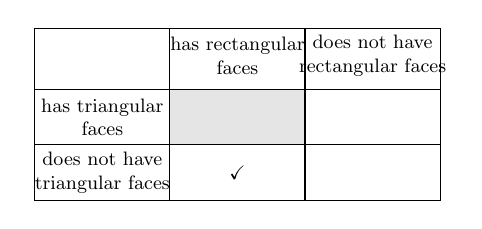
\begin{tikzpicture}[scale=0.78, every node/.style={font=\small, transform shape}]
			\draw (0,0) rectangle (6.6,2.8);
			\draw (2.2,0) -- (2.2,2.8);
			\draw (4.4,0) -- (4.4,2.8);
			\draw (0,0.9) -- (6.6,0.9);
			\draw (0,1.8) -- (6.6,1.8);
			
			\fill[gray!20] (2.2,0.9) rectangle (4.4,1.8);
			\draw (2.2,0.9) rectangle (4.4,1.8);
			
			\node[align=center] at (3.3,2.35) {has rectangular\\faces};
			\node[align=center] at (5.5,2.35) {does not have\\rectangular faces};
			
			\node[align=center] at (1.1,1.35) {has triangular\\faces};
			\node[align=center] at (1.1,0.45) {does not have\\triangular faces};
			
			\node at (3.3,0.45) {\(\checkmark\)};
		\end{tikzpicture}}
		& \CellCenter{2.5cm}{1} &
		&
		Accept any clear indication. \\
		\hline
		
		\CellCenter{\QFourHeight}{21(b)} &
		\CellCenter{\QFourHeight}{\begin{tabular}[t]{@{}p{7.2cm}@{}}
			Accept any correct shape with both rectangular and triangular faces, e.g.\ rectangular based pyramid or a triangular prism with rectangular sides. \\[0.4em]
			\centering
			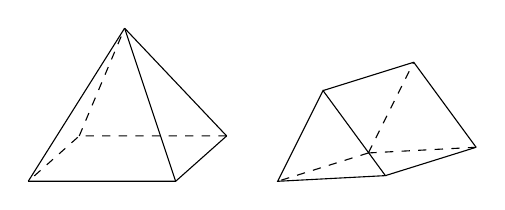
\begin{tikzpicture}[scale=0.72, every node/.style={font=\small, transform shape}]
				\coordinate (A) at (0,0);
				\coordinate (B) at (2.6,0);
				\coordinate (C) at (3.5,0.8);
				\coordinate (D) at (0.9,0.8);
				\coordinate (P) at (1.7,2.7);
				
				\draw (A) -- (B) -- (C);
				\draw[dashed] (C) -- (D) -- (A);
				
				\draw (A) -- (P);
				\draw (B) -- (P);
				\draw (C) -- (P);
				\draw[dashed] (D) -- (P);
				
				\begin{scope}[shift={(4.4,0)}]
					\coordinate (A) at (0,0);
					\coordinate (B) at (0.8,1.6);
					\coordinate (C) at (1.9,0.1);
					
					\coordinate (D) at (1.6,0.5);
					\coordinate (E) at (2.4,2.1);
					\coordinate (F) at (3.5,0.6);
					
					\draw (A) -- (B) -- (C) -- cycle;
					\draw (B) -- (E);
					\draw (C) -- (F);
					\draw (E) -- (F);
					\draw[dashed] (D) -- (A);
					\draw[dashed] (D) -- (E);
					\draw[dashed] (D) -- (F);
				\end{scope}
			\end{tikzpicture}
		\end{tabular}}
		& \CellCenter{\QFourHeight}{1} &
		&
		Accept slight inaccuracies provided the intention is clear.
		
		\vspace{0.2cm}
		Accept squares in place of rectangles.
		
		\vspace{0.2cm}
		Accept correct shape drawn in the shaded area. \\
		\hline
		
		\CellCenter{3.5cm}{22 } &
		\CellCenter{3.5cm}{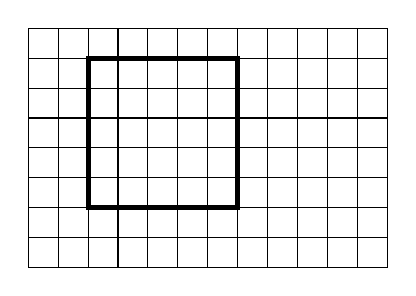
\begin{tikzpicture}[scale=0.38, every node/.style={font=\small, transform shape}]
			\draw[step=1] (0,0) grid (12,8);
			\draw[line width=1.8pt] (2,2) rectangle (7,7);
		\end{tikzpicture}}
		&\CellCenter{3.5cm}{ 1 } &
		&
		A square measuring \(5\times5\) drawn anywhere on the grid.
		
		\vspace{0.2cm}
		Accept slight inaccuracies provided the intention is clear. \\
		\hline
		
		23 &
		\begin{tabular}{|p{4.6cm}|c|c|}
			\cline{2-3}
			\multicolumn{1}{c|}{} & \textbf{true} & \textbf{false} \\
			\hline
			More people visit Animal Park than Cinema Park on Friday. & & \(\checkmark\) \\
			\hline
			Both Downtown Park and Magical Park have the same total number of visitors, on Friday and Saturday. & \(\checkmark\) & \\
			\hline
			Animal Park has the greatest \textbf{total} number of visitors. & \(\checkmark\) & \\
			\hline
			Cinema Park was the \textbf{least} popular park on Saturday. & & \(\checkmark\) \\
			\hline
		\end{tabular}
		& 2 &
		Award 1 mark for any \textbf{three} correct ticks.
		&
		Accept any clear indication. \\
		\hline
		
	\end{tabular}
	
\end{document}